\documentclass[tikz, border=2mm]{standalone}
\usepackage{amsmath}

% TikZ-Bibliotheken laden
\usetikzlibrary{decorations.pathreplacing, arrows.meta, positioning}

\begin{document}
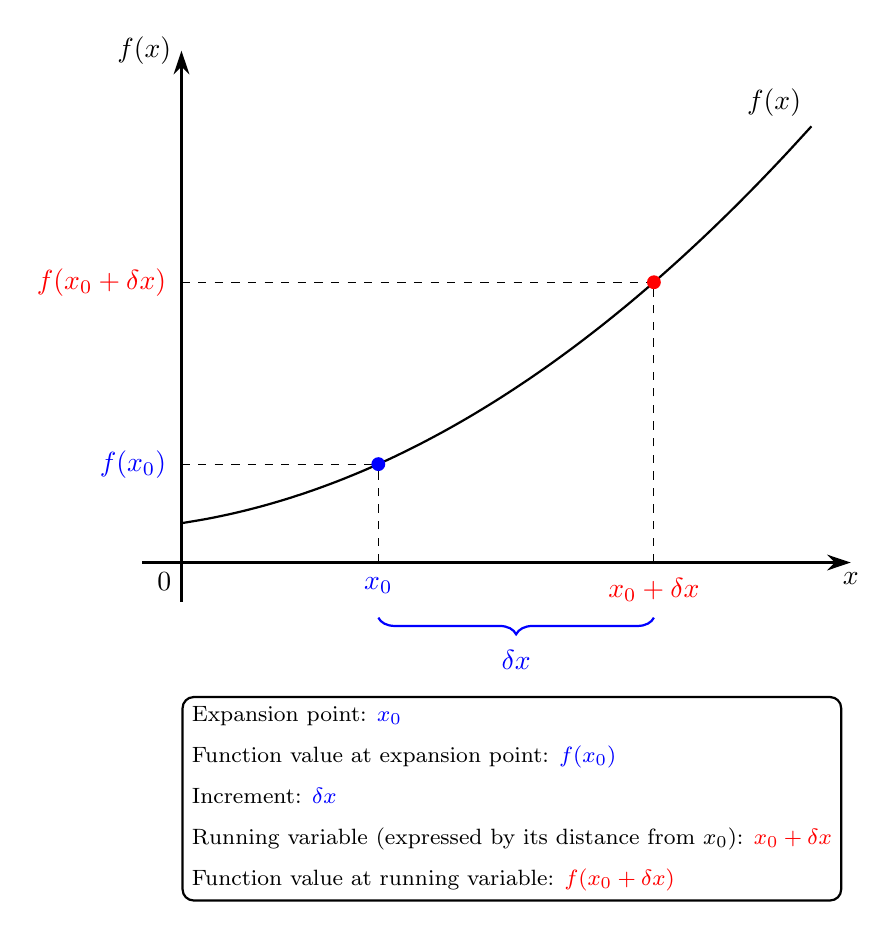
\begin{tikzpicture}[
    thick,
    >={Stealth[length=3mm, width=2mm]}, 
    declare function={f(\x) = 0.5 + 0.15*\x + 0.06*\x^2;}
]

% --- Achsen ---
\draw[->] (-0.5, 0) -- (8.5, 0) node[below] {$x$};
\draw[->] (0, -0.5) -- (0, 6.5) node[left] {$f(x)$};
\node[below left] at (0,0) {$0$};

% --- Die Funktion ---
\draw[thick, domain=0:8, smooth] plot (\x, {f(\x)}) node[above left] {$f(x)$};

% --- Definition der Punkte ---
\def\xO{2.5}         % x_0
\def\dx{3.5}         % delta x
\def\xN{\xO + \dx}   % x_0 + delta x

% Koordinaten berechnen und speichern
\coordinate (P0) at (\xO, {f(\xO)});
\coordinate (P1) at (\xN, {f(\xN)});

% --- Punkt 1 (x_0) in Blau ---
\draw[dashed, thin] (\xO, 0) node[below=2pt, text=blue] {$x_0$} -- (P0);
\draw[dashed, thin] (0, {f(\xO)}) node[left=2pt, text=blue] {$f(x_0)$} -- (P0);
\fill[blue] (P0) circle (2.5pt);

% --- Punkt 2 (x_0 + \delta x) in Rot ---
\draw[dashed, thin] (\xN, 0) node[below=2pt, text=red] {$x_0 + \delta x$} -- (P1);
\draw[dashed, thin] (0, {f(\xN)}) node[left=2pt, text=red] {$f(x_0 + \delta x)$} -- (P1);
\fill[red] (P1) circle (2.5pt);

% --- Die geschweifte Klammer für \delta x ---
\draw[decorate, decoration={brace, amplitude=6pt, mirror}, blue] 
    (\xO, -0.7) -- (\xN, -0.7) node[midway, below=8pt] {$\delta x$};

% --- The Legend Box ---
\node[draw, rounded corners, align=left, fill=white, right] at (0, -3) {
    \footnotesize Expansion point: \textcolor{blue}{$x_0$} \\[1mm]
    \footnotesize Function value at expansion point: \textcolor{blue}{$f(x_0)$} \\[1mm]
    \footnotesize Increment: \textcolor{blue}{$\delta x$} \\[1mm]
    \footnotesize Running variable (expressed by its distance from $x_0$): \textcolor{red}{$x_0 + \delta x$} \\[1mm]
    \footnotesize Function value at running variable: \textcolor{red}{$f(x_0 + \delta x)$}
};

\end{tikzpicture}
\end{document}
